\documentclass[reprint, english,notitlepage,nofootinbib]{revtex4-1}  % defines the basic parameters of the document
% if you want a single-column, remove reprint

% allows special characters (including æøå)
\usepackage[utf8]{inputenc}
%\usepackage [norsk]{babel} %if you write norwegian
\usepackage[english]{babel}  %if you write english


%% note that you may need to download some of these packages manually, it depends on your setup.
%% I recommend downloading TeXMaker, because it includes a large library of the most common packages.

\usepackage{physics,amssymb}  % mathematical symbols (physics imports amsmath)
\usepackage{graphicx}         % include graphics such as plots
\usepackage{xcolor}           % set colors
\usepackage{hyperref}         % automagic cross-referencing (this is GODLIKE)
\usepackage{tikz}             % draw figures manually
\usepackage{listings}         % display code
\usepackage{subfigure}        % imports a lot of cool and useful figure commands
\usepackage{verbatim}
\usepackage{adjustbox}


% defines the color of hyperref objects
% Blending two colors:  blue!80!black  =  80% blue and 20% black
\hypersetup{ % this is just my personal choice, feel free to change things
    colorlinks,
    linkcolor={red!50!black},
    citecolor={blue!50!black},
    urlcolor={blue!80!black}}

%% Defines the style of the programming listing
%% This is actually my personal template, go ahead and change stuff if you want
\lstset{ %
	inputpath=,
	backgroundcolor=\color{white!88!black},
	basicstyle={\ttfamily\scriptsize},
	commentstyle=\color{magenta},
	language=Python,
	morekeywords={True,False},
	tabsize=4,
	stringstyle=\color{green!55!black},
	frame=single,
	keywordstyle=\color{blue},
	showstringspaces=false,
	columns=fullflexible,
	keepspaces=true}

\newcommand\numberthis{\addtocounter{equation}{1}\tag{\theequation}}
\newcommand{\ihat}{\boldsymbol{\hat{\textbf{\i}}}}
\newcommand{\jhat}{\boldsymbol{\hat{\textbf{\j}}}}
\newcommand{\khat}{\boldsymbol{\hat{\textbf{k}}}}
\newcommand{\del}[1]{\textbf{#1)}}
\newcommand{\svar}[1]{\underline{\underline{{#1}}}}
\newcommand{\vc}[1]{\mathbf{#1}}

\graphicspath{{../output/}} % search for figures in this dir



\begin{document}


\begin{titlepage}
	\begin{center}
	\textbf{Studies of phase transitions in magnetic systems}

	\vspace{0.2cm}
	Vegard Falmår and Sigurd Sørlie Rustad

	\vspace{0.5cm}
	
\includegraphics[scale=0.5]{../../pictures/UIO}
	\vspace{0.8cm}

	University of Oslo\\
	Norway\\
	\today	\\
	\end{center}
	\tableofcontents
	\clearpage
\end{titlepage}

\begin{abstract}

\end{abstract}
\maketitle                              % creates the title


\section{Introduction}

A phase transition is when a substance changes macroscopic property because of a change in for example temperature. This can have dramatic effects, like the Meissner effect, where at a certain critical temperature superconductors become very diamagnetic (susceptibility in the order of  negative $10^5$). In this report, we are going to study the phase transition of two dimensional lattices using the Icing model and Monte Carlo simulations. In the theory section you will find a short description of the theory needed in the report. We also list some calculations and ways we have optimized our code in the appendix.

In order to make sure our code runs correctly, we test it. For a 2x2 lattice we can find analytical terms for susceptibility, heat capacity for constant volume, mean energy and mean absolute magnetization. Using this, we can compare our algorithm with analytical results, for different temperatures.

Before we study phase transitions, we also need to know how many Monte Carlo iterations we need, before we reach equilibrium. Using a 20x20 lattice and temperatures $T = 1.0, 2.4 J/k_B$, we plot mean energy and magnetization as a function of cycles. Then we can eyeball how many iterations we need to reach the most likely state. We also make a plot of the total number of accepted configurations, expecting it to drop off as we reach the most likely state.

ANALYZING THE PROBABILITY DISTRIBUTION

PHASE TRANSITION

For our studies we have used c++ for heavy computation, python for visualization and bash for automation. All the code along with instructions on how to run it, can be cloned from our GitHub repository here\footnote{github.com/sigurdru/FYS3150/tree/master/Project3}.

\section{Theory}

\subsection*{Statistical terms}
In this report we are going to use some basic statistical terms and expressions. For those not familiar with terms like standard deviation and mean value, they are covered below.

The expectation value or mean value, often written as $\left<A\right>$, is the sum of all values $A_i$, divided by the total number $N$ of values it can have:
\begin{equation*}
	\left< A \right> = \frac{1}{N}\sum_{i}^{N}A_i
\end{equation*}
However, when given a probability distribution $P_i$, which describes the probability of having outcome $A_i$, one can also find the expectation value through
\begin{equation*}
	\left<A\right> = \sum_{i}^{N}A_iP_i.
\end{equation*} 

Variance or standard deviation ($\sigma_A$), is a measurement of the variation in a set of data $A_i$. The mathematical expression is given as
\begin{equation*}
	\sigma_A = \sqrt{\frac{1}{N-1} \sum_{i}^{N} (A_i - \left<A\right>)^2} = \sqrt{\left<A^2\right> - \left<A\right>^2},
\end{equation*} 
where $N$ is the total number of outcomes and $\left<A\right>$ is the expectation value of $A_i$.

\subsection*{Monte Carlo}

Monte Carlo simulations is a broad term for algorithms that rely on random sampling. An example of this is using Monte Carlo simulations to approach the value of pi\footnote{https://academo.org/demos/estimating-pi-monte-carlo/}. We are going to use it to chose and flip spins in our lattice.

Lets say we have a $L$x$L$ lattice, with $L^2$ spins. One Monte Carlo cycle entails choosing $L^2$ spins at random and flipping it based on the probability described by equation \eqref{eq:prob_flip}. Each cycle we can calculate the energy and magnetization. The idea is that after a large $N$ number of cycles, we have reached a state with properties like that of a physical one. The challenge here is having the right probability distribution and completing enough cycles $N$.

\subsection*{Canonical ensemble}
The probability of finding a system in a given microstate is found through the canonical ensemble, given by equation \eqref{eq:canonical_ensemble} (see \cite{lectures2015} chapter 13.2.2).
\begin{equation}
	\label{eq:canonical_ensemble}
	P_i(\beta) = \frac{\exp(-\beta E_i)}{Z},\ \ \beta = \frac{1}{k_BT}
\end{equation}
Here $P_i(\beta)$ is the probability of finding the system with energy $E_i$ and temperature $T$ in Kelvin. $k_B$ is Boltzmann constant and $Z$ the partition function given by
\begin{equation}
	\label{eq:partition_function}
	Z = \sum_{i = 1}^{M}\exp(-\beta E_i).
\end{equation}
Where $M$ is the total number of microstates.

The canonical ensemble and partition function is usually hard to find, however, when obtained we can use them to find many useful relations. Below we list the expressions (without derivation) we need will need in the report. Everything is from \cite{lectures2015} chapter 13.2.2.

The mean energy $\left<E\right>$ given as
\begin{equation}
	\label{eq:expected_energy}
	\left<E\right> = \frac{1}{Z} \sum_{i=1}^{M}E_i\exp(-\beta E_i),
\end{equation}
and the mean square energy ($\left<E^2\right>$) is calculated by
\begin{equation}
	\label{eq:expected_energy_sq}
	\left<E^2\right> = \frac{1}{Z} \sum_{i=1}^{M}E_i^2\exp(-\beta E_i).
\end{equation}
Mean absolute value of the magnetic moment $\left<|M|\right>$
\begin{equation}
	\label{eq:expected_magnetic_moment}
	\left<|M|\right> = \frac{1}{Z} \sum_{i=1}^{M}|M_i|\exp(-\beta E_i),
\end{equation}
and mean square magnetic moment ($\left<M^2\right>$) by
\begin{equation}
\label{eq:expected_magnetic_moment_sq}
\left<M^2\right> = \frac{1}{Z} \sum_{i=1}^{M}M_i^2\exp(-\beta E_i).
\end{equation}
With this we can also find the susceptibility $\chi$
\begin{equation}
	\label{eq:magnetic_susceptibility}
	\chi = \beta \sigma^2_M, \ \ \sigma_M = \sqrt{\left<M^2\right> - \left<|M|\right>}
\end{equation}
Where $\sigma_M$ is the variance of $|M|$. We evaluate the absolute value of $M$ because that gives nicer plots. Specific heat capacity at constant volume $C_V$ is given by
\begin{equation}
	\label{eq:specific_heat_capacity}
	C_V = \frac{\beta}{T}\sigma^2_E, \ \ \sigma_E = \sqrt{\left<E^2\right> - \left<E\right>}
\end{equation}
$\sigma_E$ is the variance of $E$.

\subsection*{Icing model for two dimensional lattice} \label{sect:2by2Lattice}

From \cite{oppgavetekst} the energy in a 2D lattice with no external magnetic field is given by
\begin{equation}
	\label{eq:2D_energy}
	E = -J \sum_{<kl>}^{N}s_ks_l,
\end{equation}
where $s_k = \pm 1$ (representing the spin direction), $N$ the total number of spins and $J$ a coupling constant indicating the strength of the interaction between neighboring spins. The $<kl>$ means that we sum over the nearest neighbors.

Her dekker vi prob for flip
\begin{equation}
	\label{eq:prob_flip}
	A = B
\end{equation}

\subsection*{Phase transitions}

A phase transition is an abrupt change on the macroscopic scale (i.e. ice melting), because parameters like pressure and temperature changing. The point at which this happens is called the critical point. In this report we are going to study the critical temperature ($T_C$), and will cover some theory and necessary equations for our report. Everything is from \cite{lectures2015} chapter 13, and we recommend reading it for a more extensive explanation.

In our simulations we expect to see a second order transition at critical temperature. Meaning mean magnetization $\left<M>\right>$ will go from zero to not be zero. For critical phenomena, when temperature approaches critical ($T\rightarrow T_C$) the mean magnetic moment ($\left<M(T)\right>$) scales as (for $T<T_C$)
\begin{equation}
	\label{eq:critical_M}
 	\left<M(T)\right> \sim \left(T - T_C\right)^{1/8},
\end{equation}
susceptibility ($\chi(T)$) scales as
\begin{equation}
	\label{eq:critical_chi}
	\chi(T) \sim \abs{T_C - T}^{7/4}
\end{equation}
and specific heat capacity ($C_V$) as
\begin{equation}
	\label{eq:critical_Cv}
	C_V(T) \sim \abs{T_C - T}^0.
\end{equation}
The exponents are what we refer to as critical exponents.

Another relation we can find is correlation length ($\xi$), which describes the length scale when overall properties of the material starts to differ from its bulk properties. When $T\geqq T_C$ it is at the length scale of the lattice spacing. When we approach critical temperature spins become more correlated, and when the they are close, the correlation length goes as
\begin{equation}
	\label{eq:critical_ksi}
	\xi(T) \sim \abs{T_C - T}^\nu.
\end{equation}
Where $\nu$ is another critical exponent, which we will set to $\nu=1$ in our report.

\section{Methods}

As we mentioned in the introduction, in this report we are going to simulate a 2D lattice with $L^2$ number of spins, $L$ in the x- and y-direction. We will look at different numbers of spin and temperature, looking at how our system responds. We are only going to use periodic boundary conditions, meaning the edges are neighbors. For a square peace of (stretchy) paper, this would look like first folding it into a cylinder and then into a donut-shape. We are going to use random initial spin direction, unless we specify otherwise. To simulate we are going to use Monte Carlo simulations for choosing and flipping spins. We use the probability distribution described by equation \eqref{eq:prob_flip} to choose weather or not to flip spins (see the theory section for a more detailed description).



\subsection{Units}

We scale our units in order to have easier numbers to work with. We use J and the Boltzmann constant $k_B$, such that we get the units described by table \ref{tab:units}.

\begin{table}[h]
	\begin{tabular}{||l|l||}
		\hline
		Quantity             & Unit   \\
		\hline
		Energy ($E$)              & J      \\
		\hline
		Magnetization ($M$)        & $-$      \\
		\hline
		Temperature ($T$)        & J/$k_B$ \\
		\hline
		Susceptibility ($\chi$ ) & 1/J   \\
		\hline
	\end{tabular}
	\caption{Table showing the units we use in this report, after scaling.}
	\label{tab:units}
\end{table}

\subsection{Testing of algorithm}

In order to make sure our algorithm is running correctly, we want to test it. We do this by comparing it to analytical results, namely a 2x2 lattice.

By using equation \eqref{eq:2D_energy} and testing all 16 different combinations for a 2D lattice, we have made a table \ref{tab:E_and_M_2D_lattice} that shows all the possible energies and magnetizations, as well as the multiplicity of each configuration (marked as degeneracy).
\begin{table}[h]
	\input{tables/tab_E_and_M_2D_tex.txt}
	\caption{Table showing the energy, multiplicity and magnetization of different configurations of spins in a $2 \times 2$ 2D-lattice with periodic boundary conditions.}
	\label{tab:E_and_M_2D_lattice}
\end{table}
With this we can find the analytical term of the partition function ($Z$). Reading the values from table \ref{tab:E_and_M_2D_lattice} and using equation \eqref{eq:partition_function} we get:
\begin{align*}
Z &= \sum_{i = 1}^{16} \exp(-\beta E_i) \\
&= 12 + 2\exp(8\beta) + 2\exp(-8\beta) \\
&= 12 + 4\cosh(8\beta). \numberthis \label{eq:2Dpartition_function}
\end{align*}
With the partition function and the canonical ensemble through equation \eqref{eq:canonical_ensemble}, we can find a lot of useful values. With equations (\ref{eq:expected_energy}-\ref{eq:specific_heat_capacity}) we obtain energy $\left<E\right	>$, mean absolute value of the magnetic moment $\left<|M|\right>$, susceptibility $\chi$ and specific heat capacity at constant volume $C_V$. The calculations are done in the appendix \ref{calc_of_22_lattice}.

With this we can compare our simulations to expected theoretical values. Plotting expectation values (for $T=1$J/$k_B$) as a function of Monte Carlo iterations we can get an idea of how many we need to reach equilibrium. Then we can plot simulated and theoretical expectation values as a function of temperature, to see how well they correspond. Ideally we want them to overlap completely.

\subsection{Reaching the most likely state (denne må finskrives)}
From looking at an 2x2 lattice, we will get an idea of how many Monte Carlo cycles we will need to reach equilibrium. However we want to study this more carefully, testing for $L=20$ spins. First with a temperature of $T = 1 $J$/K_B$, then $T = 2.4 $J$/K_B$, we will plot the expectation value of energy ($\left<E\right>$) and absolute magnetization ($\left<|M|\right>$) as a function of iterations. After testing with random initial conditions, we also do the same looking spin starting in the same direction. 

We also want to study the number of accepted configurations. This means we want to count the number of times we flip a spin. We therefore make a plot of the total number of accepted configurations as a function of iterations. We also look at how this varies with temperature.

It is interesting what the probability of obtaining an energy $E$ is (like a numerical partition function). The way we do this, is by finding out how many times a given energy $E$ appears and then divide it by the total number of energies tested for. Then we will get an estimate of the probability one energy appears. Then compare it to the computed variance in energy ($\sigma_E$). 

\subsection{Study of phase transition}

First we look at how our system behaves for different lattice sizes, around critical temperature. We test for $L=40$, $L=60$, $L=80$ and $L=100$ in the temperature range $T[K_B/J]\in [2.0, 2.3]$. We will initially start with a temperature step of $\Delta T = 0.005$, however might change it based on results. For the different lattice sizes we will plot $\left<E\right>$, $\left<|M|\right>$, $C_V$ and $\chi$ as a function of temperature $T$. Our hope is that we can see an indication of a phase transition, namely a changes in traits around a specific temperature.

\section{Results}

In figure \ref{fig:L2_T1_Random_and_not} you find theoretical and computed values for $\left<E\right>$, $\left<|M|\right>$, $C_V$ and $\chi$, in a 2x2 lattice. Both with random (top four plots) initial values, and ordered (all spins starting in the same direction) initial conditions (bottom four plots).

Similar plots can be found for the 20x20 lattice in figure \ref{fig:L20_T1_and_T2_4}. There we have plotted the computed values of $\left<E\right>$, $\left<|M|\right>$, $C_V$ and $\chi$, where the top four are for the temperature $T=1$ and the bottom four are for $T=2.4J/k_B$. 

We also plotted the number of accepted configurations as a function of Monte Carlo Cycles in figure \ref{fig:Num_flips_T1_and_T2_4}. The top two plots are for temperature $T=1J/k_B$, with both random and ordered initial configuration, and the bottom two are with temperature $T=2.4J/k_B$.

\begin{figure*}[!htb]
	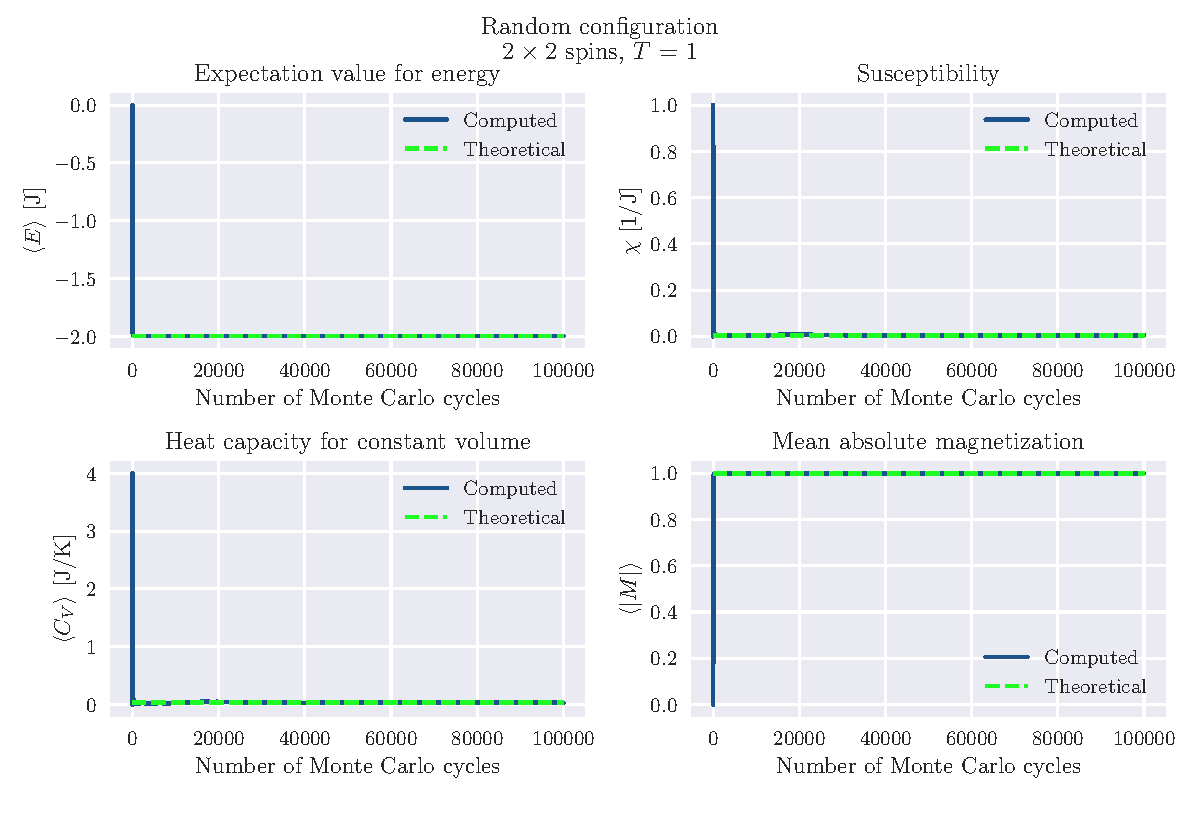
\includegraphics[width=16cm]{../output/c/L2-T1-dT0_0-NT1-N5-RandomTrue_comp.pdf}
	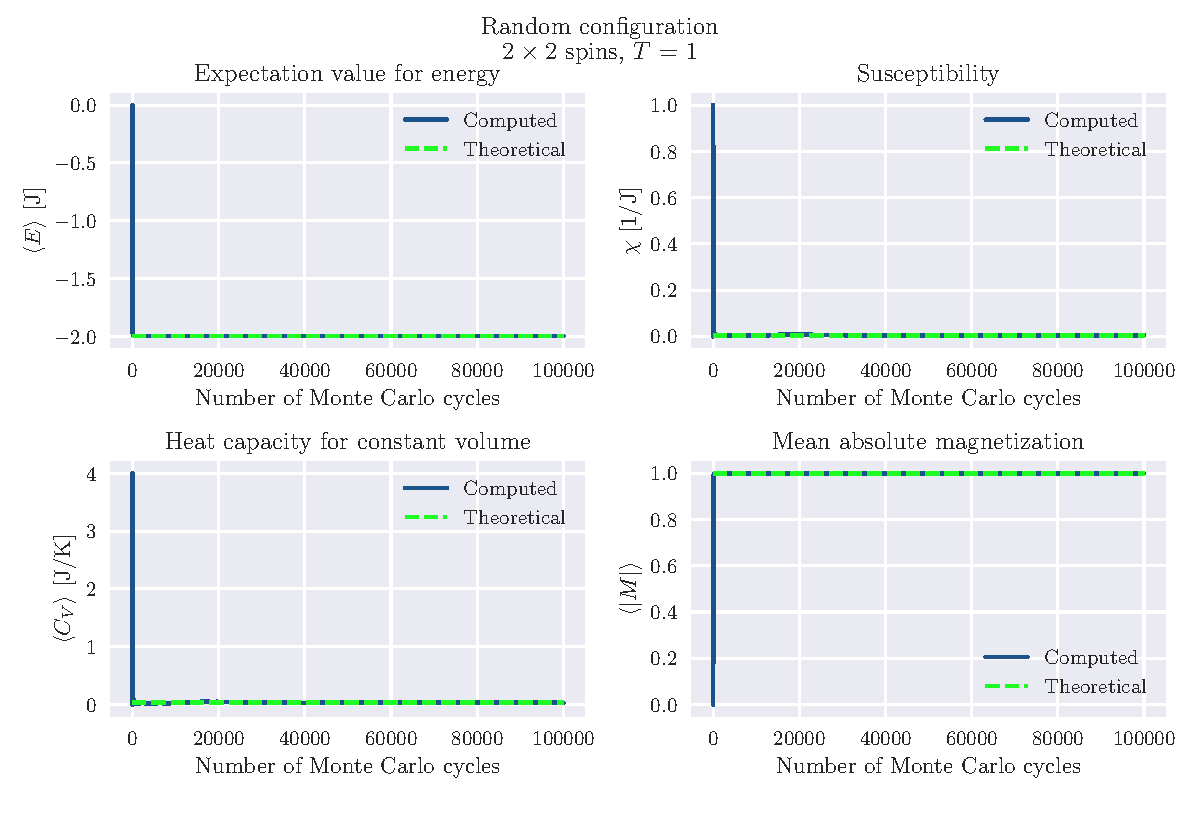
\includegraphics[width=16cm]{../output/c/L2-T1-dT0_0-NT1-N5-RandomTrue_comp.pdf}
	\caption{In this figure you see the theoretical and computed values of $\left<E\right>$, $\left<|M|\right>$, $C_V$ and $\chi$, for a 2x2 lattice and temperature $T=1J/k_B$. The top four plots are from random initial values, and the bottom four are from all pointing in the same direction.} 
	\label{fig:L2_T1_Random_and_not}
\end{figure*}
\begin{figure*}[!htb]
	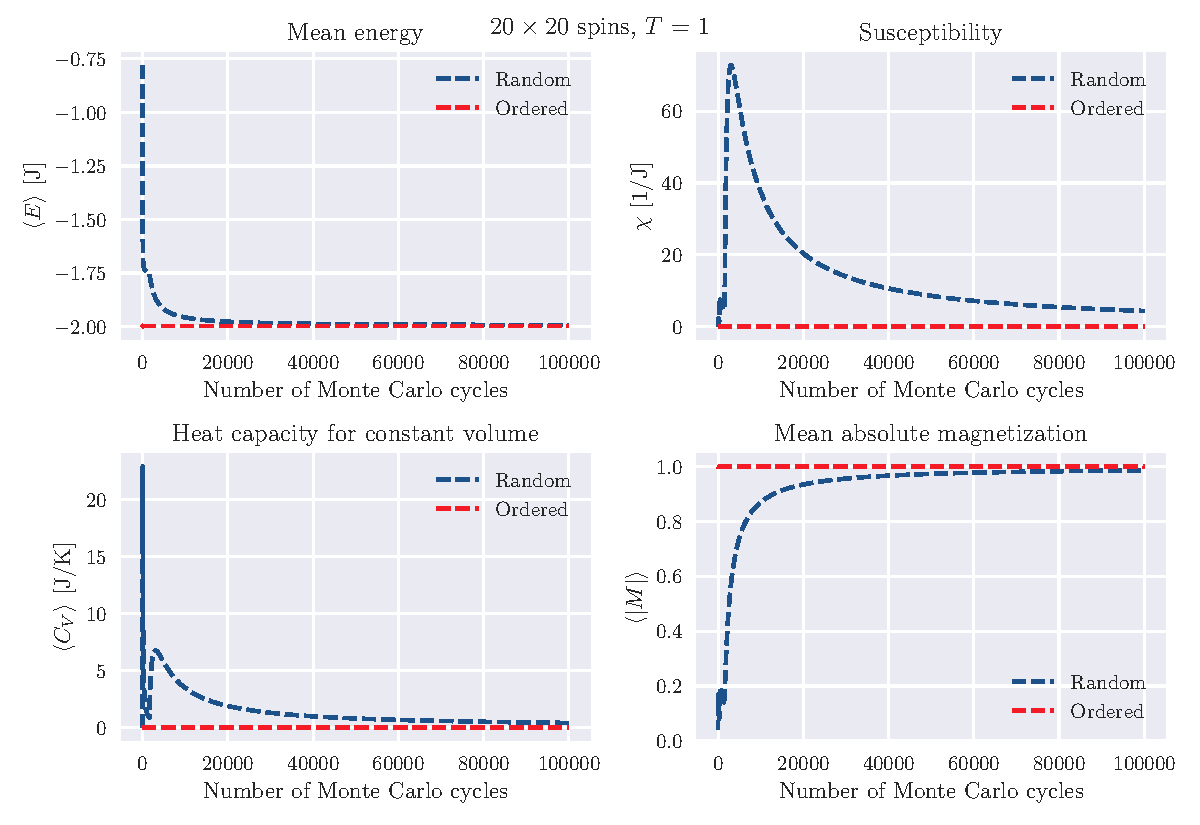
\includegraphics[width=16cm]{../output/de/L20-T1-dT0_0-NT1-N5-ExpVals.pdf}
	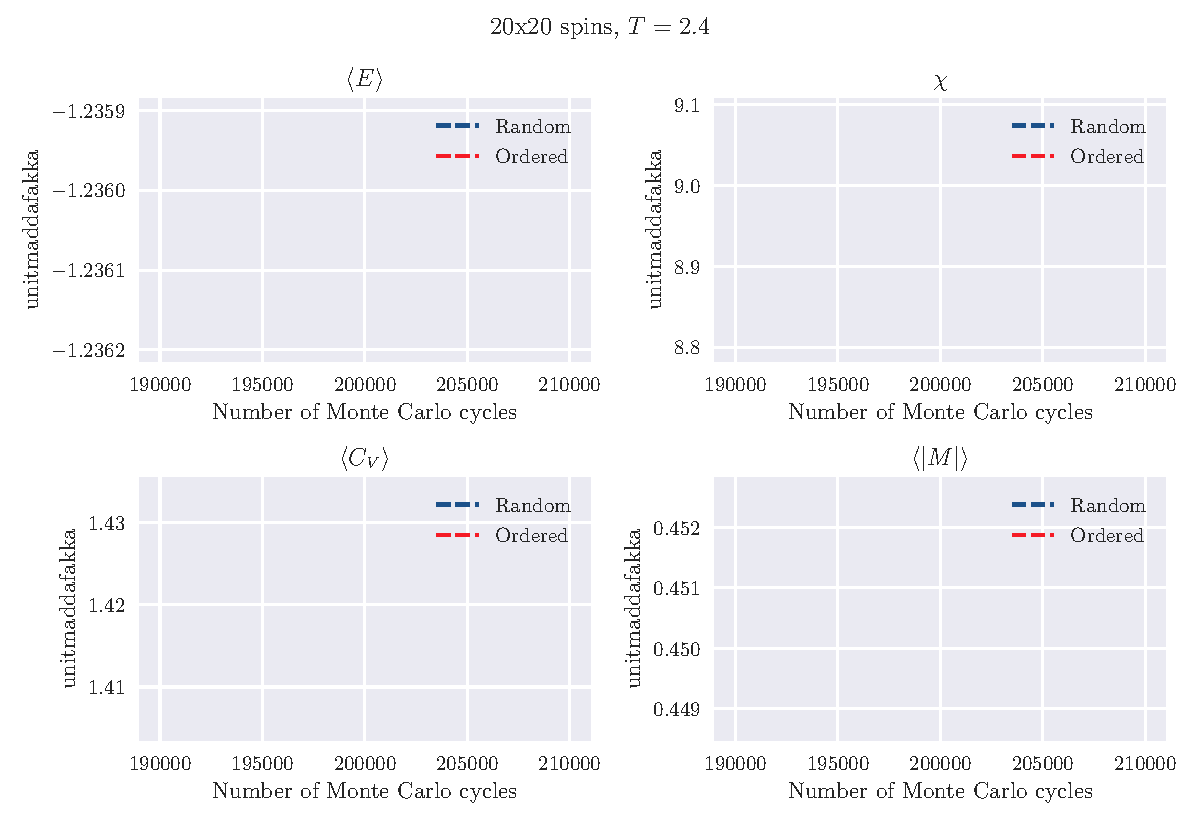
\includegraphics[width=16cm]{../output/de/L20-T2_4-dT0_0-NT1-N5-ExpVals.pdf}
	\caption{In this figure you see the computed values of $\left<E\right>$, $\left<|M|\right>$, $C_V$ and $\chi$, for both random and ordered initial conditions. The top four shows the computed values for random and ordered initial conditions, for a temperature $T=1J/k_B$. Bottom four shows the same, only for a temperature $T=2.4J/k_B$.}
	\label{fig:L20_T1_and_T2_4}
\end{figure*}
\begin{figure*}[!htb]
	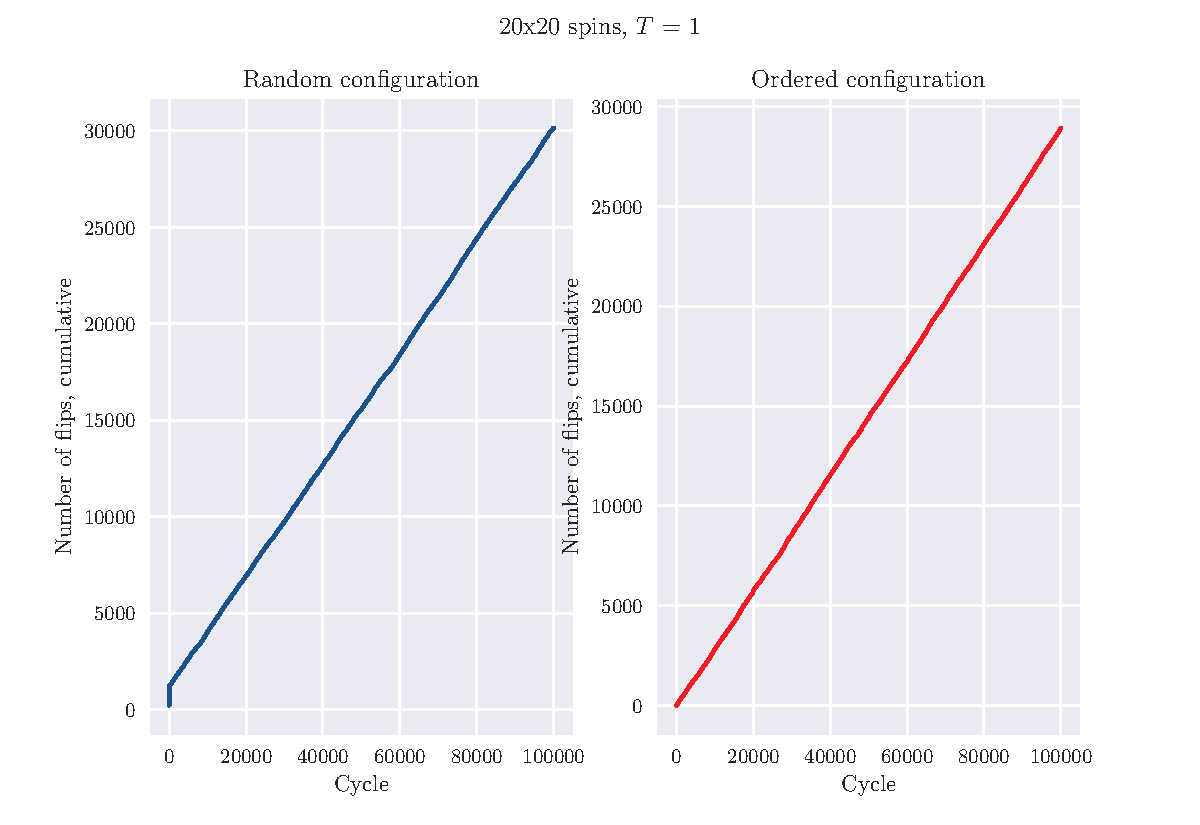
\includegraphics[width=16cm]{../output/de/L20-T1-dT0_0-NT1-N5-NumSpins.pdf}
	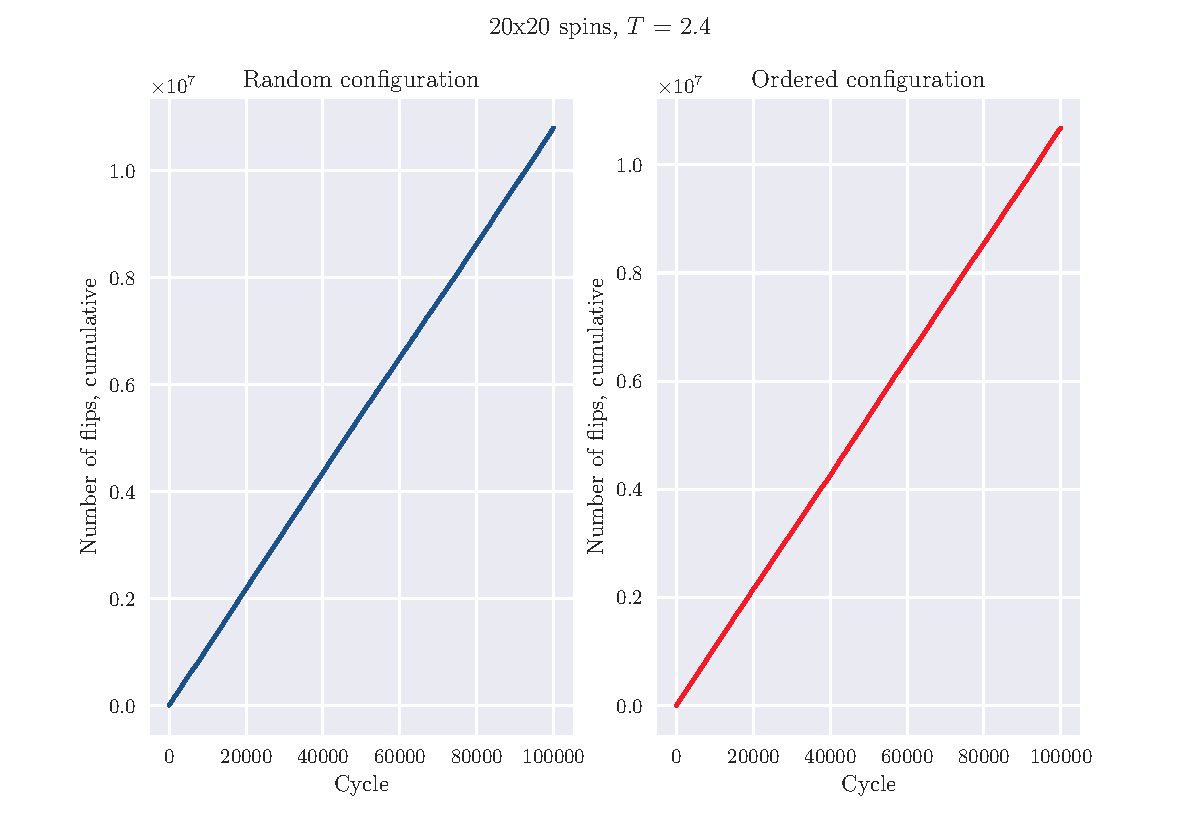
\includegraphics[width=16cm]{../output/de/L20-T2_4-dT0_0-NT1-N5-NumSpins.pdf}
	\caption{Here we have plotted the number of accepted configuration as a function of Monte Carlo cycles, for a 20x20 lattice. The top two plots are with temperature $T=1J/k_B$, and shows both random and ordered initial conditions. The bottom two shows the same, only with a temperature of $T = 2.4$.}
	\label{fig:Num_flips_T1_and_T2_4}
\end{figure*}

\section{Discussion}

slette første delen av data

\section{Appendix}
\subsection{Algorithm specific optimization}

In order to make our algorithm run faster, we do some optimization. We list the optimizations we implemented here, to make our code easier to understand and as a guide for anyone who wants to do something similar.

During our simulations we calculate the change in energy ($\Delta$E) many times. We want to make more efficient by exploring the possible values $\Delta E$ can have. During our simulations we only evaluate one spin at a time, meaning we only need to look at the possible values $\Delta E$ can have when flipping one spin. It turns out there are five possible situations (using equation \eqref{eq:2D_energy}):
\begin{align*}
	\text{Zero down: } &\begin{matrix}
	& \uparrow  \\
	\uparrow & \uparrow & \uparrow \\
	& \uparrow
	\end{matrix}
	\rightarrow	
	\begin{matrix}
	& \uparrow  \\
	\uparrow & \downarrow & \uparrow \\
	& \uparrow
	\end{matrix}
	\implies
	\Delta E = 8J \\
	\text{One down: }
		&\begin{matrix}
	& \downarrow  \\
	\uparrow & \uparrow & \uparrow \\
	& \uparrow
	\end{matrix}
	\rightarrow	
	\begin{matrix}
	& \downarrow  \\
	\uparrow & \downarrow & \uparrow \\
	& \uparrow
	\end{matrix}
	\implies
	\Delta E = 4J \\
	\text{Two down: }
		&\begin{matrix}
	& \downarrow  \\
	\downarrow & \uparrow & \uparrow \\
	& \uparrow
	\end{matrix}
	\rightarrow	
	\begin{matrix}
	& \downarrow  \\
	\downarrow & \downarrow & \uparrow \\
	& \uparrow
	\end{matrix}
	\implies
	\Delta E = 0J \\
	\text{Three down: }
		&\begin{matrix}
	& \downarrow  \\
	\downarrow & \uparrow & \downarrow \\
	& \uparrow
	\end{matrix}
	\rightarrow	
	\begin{matrix}
	& \downarrow  \\
	\downarrow & \downarrow & \downarrow \\
	& \uparrow
	\end{matrix}
	\implies
	\Delta E = -4J \\
	\text{Four down: }
		&\begin{matrix}
	& \downarrow  \\
	\downarrow & \uparrow & \downarrow \\
	& \downarrow
	\end{matrix}
	\rightarrow	
	\begin{matrix}
	& \downarrow  \\
	\downarrow & \downarrow & \downarrow \\
	& \downarrow
	\end{matrix}
	\implies
	\Delta E = -8J \\
\end{align*}
We can thus compute and store the different values of $e^{- \beta \Delta E}$ beforehand to avoid making these computations every time we update the energy.

As mentioned previously, we are going to use periodic boundary conditions. The easiest, but slow way of implementing this, is with if-tests. However we did it with a simple function (in c++),
\begin{lstlisting}
int PeriodicBoundary(int i, int limit, int add) { 
	return (i+limit+add) % (limit);
}
\end{lstlisting}
that takes the current index you are evaluating (\texttt{i}), the total size (\texttt{limit}) and the amount you want to go forward and backward (\texttt{add}). Then we sum all the arguments and take the rest, reassuring us we always arrive at the right index, or if we are at the edge, wrap back around.

PARALELIZATION

\subsection{Calculations of 2x2 lattice} \label{calc_of_22_lattice}

Inserting the values from table \ref{tab:E_and_M_2D_lattice} into equations \eqref{eq:canonical_ensemble} and (\ref{eq:expected_energy}-\ref{eq:specific_heat_capacity}) we get
\begin{align*}
	\left<E\right> &= \frac{1}{Z}\left(-8Je^{8\beta} + 2\cdot 8Je^{-8\beta } - 8J e^{8\beta }\right) \\
	&= \frac{-32J}{Z}\cosh(8\beta )\\
	\left<E^2\right> &= \frac{1}{Z}\left((-8J)^2e^{8\beta J} + 2\cdot (8J)^2e^{-8\beta J} (- 8J)^2 e^{8\beta }\right) \\
	&= \frac{256J^2}{Z}\cosh(8\beta)\\
	\left<|M|\right> &= \frac{1}{Z}\left(4e^{8\beta } + 4\cdot 2e^{0} + 4\cdot 2 e^{0} + 4e^{8\beta }\right) \\
	&= \frac{8}{Z}\left(2 + e^{8\beta }\right)\\
	\left<M^2\right> &= \frac{1}{Z}\left(4^2e^{8\beta } + 4\cdot 2^2e^{0} + 4\cdot 2^2 e^{0} + 4^2e^{8\beta }\right) \\
	&= \frac{32}{Z}\left(1 + e^{8\beta }\right)\\
	\chi &= \frac{32\beta}{Z}\left(\left(1 + e^{8\beta }\right) - \frac{2}{Z}\left(2 + e^{8\beta }\right)^2 \right)\\
	C_V &= \frac{256J^2\beta}{TZ}\left(\cosh(8\beta) - \frac{4}{Z}\cosh[2](8\beta)\right)
\end{align*}


\onecolumngrid
\vspace{1cm} % some extra space

\begin{thebibliography}{}
\bibitem[]{oppgavetekst} Department of Physics, Univeristy of Oslo, Fall semester 2020, Computational Physics I FYS3150/FYS4150, Project 4.
\bibitem[]{lectures2015} Morten Hjorth-Jensen, Computational Physics, Lecture Notes Fall 2015, August 2015, https://github.com/CompPhysics/ComputationalPhysics/blob/master/doc/Lectures/lectures2015.pdf.
\bibitem[]{larsonsager} Lars Onsager, Crystal Statistics. I. A two-Dimensional Model with an Order-Disorder Transition, 1. February 1944, https://journals.aps.org/pr/abstract/10.1103/PhysRev.65.117

\end{thebibliography}


\end{document}
